\paragraph{QuizziPedia::Front-End::Controllers::TrainingController}
\begin{figure} [ht]
	\centering
	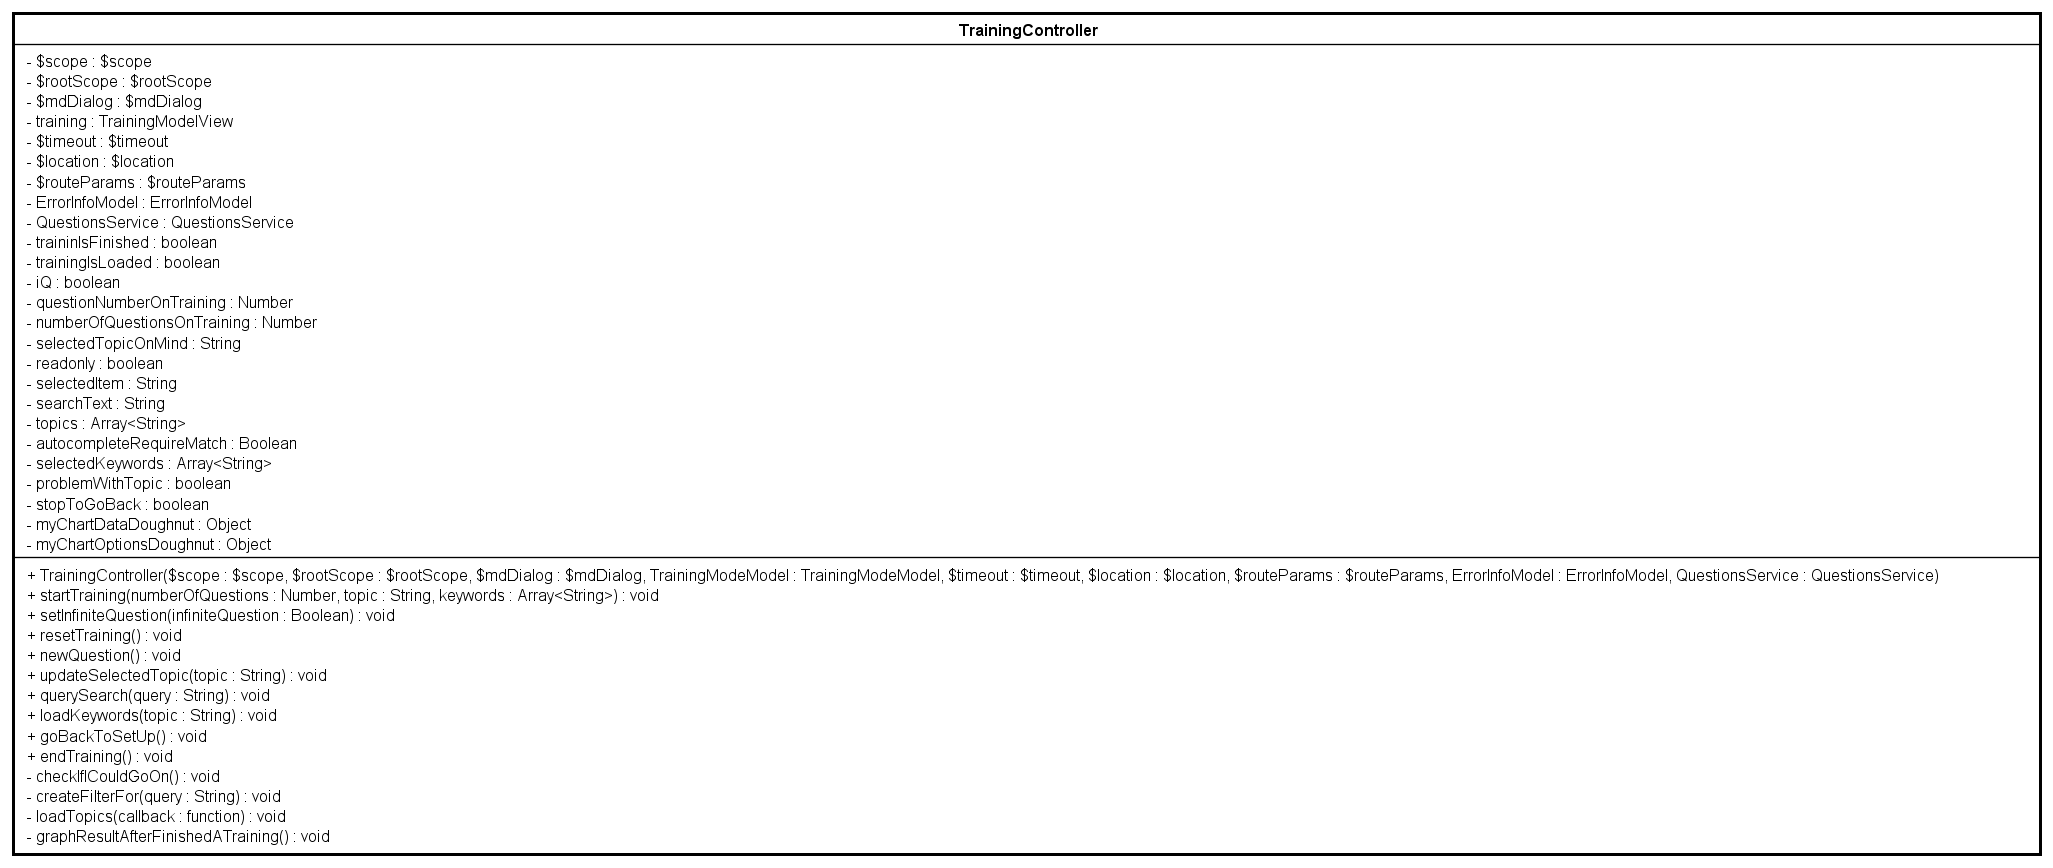
\includegraphics[scale=0.45]{UML/Classi/Front-End/QuizziPedia_Front-end_Controller_TrainingController.png}
	\caption{QuizziPedia::Front-End::Controllers::TrainingController}
\end{figure} \FloatBarrier
\begin{itemize}
	\item \textbf{Descrizione}: questa classe permette di gestire la modalità allenamento sottoponendo all'utente le giuste domande adatte al suo livello;
	\item \textbf{Utilizzo}: fornisce le funzionalità per recuperare le domande che siano in accordo con il livello dell'utente;
	\item \textbf{Relazione con altre classi}:
	\begin{itemize}
		\item \textbf{IN \texttt{TrainingModelView}}: classe di tipo \textit{modelview\ped{G}} la cui istanziazione è contenuta all'interno della variabile di ambiente \$scope di \textit{Angular\ped{G}}. All'interno di essa sono presenti le variabili e i metodi necessari per il \textit{Two-Way Data-Binding\ped{G}} tra la \textit{view\ped{G}} \texttt{TrainingView} e il \textit{controller\ped{G}} \texttt{TrainingController};
		\item \textbf{IN \texttt{TrainingModeModel}}: rappresenta un allenamento. Contiene tutte le informazioni necessarie alla presentazione del contenuto di un allenamento;
		\item \textbf{IN \texttt{QuestionController}}: questa classe permette di gestire il recupero delle domande per far si che possano essere visualizzate nella modalità allenamento e nella compilazione dei questionari.
	\end{itemize}
	\item \textbf{Attributi}:
	\begin{itemize}
		\item \texttt{-} \texttt{\$scope: \$scope} \\
		Campo dati contenente un riferimento all'oggetto \$scope creato da \textit{Angular\ped{G}}, viene utilizzato come mezzo di comunicazione tra il \textit{controller\ped{G}} e la \textit{view\ped{G}}. Contiene gli oggetti che definiscono il \textit{model\ped{G}} dell'applicazione;
		\item \texttt{-} \texttt{\$rootScope: \$rootScope} \\
		Campo dati contenente il riferimento all'oggetto globale \$rootScope creato da \textit{Angular\ped{G}}. Viene utilizzato per rendere accessibile a tutti i \textit{controller\ped{G}} e a tutte le \textit{view\ped{G}} l'oggetto \texttt{TrainingModeModel}. In questo caso viene utilizzato per inserire in \$rootScope l'oggetto di ritorno della chiamata a \texttt{getNextQuestion};
		\item \texttt{-} \texttt{\$mdDialog: \$mdDialog} \\
		Campo dati contenente un riferimento al servizio della libreria \textit{Material for Angular\ped{G}} che permette di creare delle componenti a pop-up;
		\item \texttt{+} \texttt{training: TrainingModelView} \\
		Oggetto di tipo \texttt{TrainingModelView}. All'interno di esso sono presenti le variabili e i metodi necessari per il \textit{Two-Way Data-Binding\ped{G}} tra la \textit{view\ped{G}} \texttt{TrainingView} e il \textit{controller\ped{G}} \texttt{TrainingController};
	\end{itemize}
	\item \textbf{Metodi}:
	\begin{itemize}
		\item \texttt{+} \texttt{TrainingController(\$scope: \$scope, \$rootScope: \$rootScope, \$mdDialog: \$mdDialog, TrainingModeModel: TrainingModeModel)} \\ Metodo costruttore della classe. \\
		\textbf{Parametri:}
		\begin{itemize}
			\item \texttt{\$scope: \$scope} \\
			Parametro contenente un riferimento all'oggetto \$scope creato da \textit{Angular\ped{G}}. Viene utilizzato come mezzo di comunicazione tra il \textit{controller\ped{G}} e la \textit{view\ped{G}}. Contiene gli oggetti che definiscono il \textit{viewmodel\ped{G}} e il \textit{model\ped{G}} dell'applicazione;
			\item \texttt{\$rootscope: \$rootscope}\\
			Parametro contenente il riferimento all'oggetto globale \$rootScope creato da \textit{Ang-\\ular\ped{G}}. Viene utilizzato per rendere accessibile a tutti i \textit{controller\ped{G}} e a tutte le \textit{view\ped{G}} l'oggetto \texttt{UserDetailsModel}. In questo caso viene utilizzato per aggiornare in \$rootScope l'oggetto che rappresenta l'utente autenticato all'interno dell'applicazione;
			\item \texttt{\$mdDialog: \$mdDialog} \\
			Parametro contenente un riferimento al servizio della libreria \textit{Material for Angular\ped{G}} che permette di creare delle componenti a pop-up;
			\item \texttt{TrainingModeModel: TrainingModeModel} \\ Rappresenta un allenamento. Contiene tutte le informazioni necessarie alla presentazione del contenuto di un allenamento.
		\end{itemize}
		\item \texttt{+} \texttt{addQuestion(question: QuestionItemModel): void} \\
		Metodo che gestisce l'evento per inserire una domanda nella cronologia delle domande. \\
		\textbf{Parametri}:
		\begin{itemize}
			\item \texttt{question: QuestionItemModel} \\
			Parametro contenente un riferimento all'oggetto di tipo \texttt{QuestionItemModel}.
		\end{itemize}
		\item \texttt{+} \texttt{loadNewQuestionBy(topic: String, keywords: Array<String>, level:\\ Number): void} \\
		Metodo che emette l'evento per scaricare una nuova domanda in base ai parametri passati. Fa una richiesta al \texttt{QuestionsController} che andrà a scaricare la domanda e ad inserirla in \texttt{TrainingModeModel} nello \$scope mediante il metodo \texttt{addQuestion}; \\
		\textbf{Parametri}:
		\begin{itemize}
			\item \texttt{topic: String} \\
			Parametro contenente l'argomento della domanda;
			\item \texttt{keywords: Array<String>} \\
			Parametro contenente un array di stringhe che rappresenta le keywords scelte per l'allenamento;
			\item \texttt{level: Number} \\
			Parametro contenente il livello dell'utente.
		\end{itemize}
		\item \texttt{+} \texttt{addResult(questionNumber: Number, result: Boolean): void} \\
		Metodo che gestisce l'evento per inserire il risultato di una domanda. \\
		\textbf{Parametri}:
		\begin{itemize}
			\item \texttt{questionNumber: Number} \\
			Parametro contenente il numero della domanda risposta;
			\item \texttt{result: Boolean} \\
			Parametro contenente il risultato della domanda risposta.
		\end{itemize}
		\item \texttt{+} \texttt{startTraining(numberOfQuestions: Number, topic: String, keywords:\\ Array<String>): void} \\
		Metodo che gestisce l'evento per iniziare l'allenamento. \\
		\textbf{Parametri}:
		\begin{itemize}
			\item \texttt{numberOfQuestions: Number} \\
			Parametro contenente il numero di domande per l'allenamento;
			\item \texttt{topic: String} \\
			Parametro contenente l'argomento dell'allenamento;
			\item \texttt{keywords: Array<String>} \\
			Parametro contenente un array di stringhe che rappresenta le keywords scelte per l'allenamento.
		\end{itemize}
	\end{itemize}
\end{itemize}

